\chapter{Neue Auswahlkomponenten}

\section{Design}

\subsection{Mögliche Designoptionen eines Elements}

% border, background-color, font-color, underline, italic, font-weight, line left side
% pro cons pro möglichkeit mit passenden farboptionen
% kombination 2er status eines elements


\section{Interaktionen}

Für die Bedienung der Komponente gilt es Regeln festzulegen, damit ein gemeinsames Verständis entsteht.
Wie in den Grundlagen bereits beschrieben kann sich ein Wert aus der Komponentenliste verschiedene in Zuständen befinden.
In diesem Absatz spielen Selektion, Highlight und Cursor Position eine Rolle.
Zur Auffrischung: 

\begin{itemize}
    \item \textbf{Selektion}: Ausgewählter Wert der Spalte
    \item \textbf{Highlight}: Element unterhalb des Maus Zeiger
    \item \textbf{Cursor Position}: Element-Position für die Tastatur
\end{itemize}

\noindent
Bei der Festlegung der Maus-Interaktion fiel die Entschiedung auf folgendes:

\begin{itemize}
    \item \textbf{mouseover}: visuelles Highlighting des Elements ohne Selektionsänderung
    \item \textbf{click}: wie mit der Tastatur
\end{itemize}

\noindent
Hingegen die Tastatur-Steuerung mit den Pfeiltasten hält sich an diese Bedienungen:

\begin{itemize}
    \item direkte Selektionsänderung ohne weiter Bestätigung
    \item Änderung der Cursor Position
\end{itemize}

\noindent
Anhand dieser Regeln enstanden folgendene Aktionen als Basis für den ersten Projektor der neuen Komponente. 


\clearpage
\import{../tables}{d.newComponent.tex}

Das Undo und das Redo auf der Komponente erhält im ersten Projektor keine speziell Definition.
Anders als bei den existierenden Komponenten, ist bei der neuen die Leetaste neu belegt. 
Bei der geschlossenen Komponente ist das Verhalten mit dem Öffnen der Liste teilweise übernommen.
Ist die Liste bereits offen, wird der sich aktuell unter der Cursorposition befindliche Wert selektiert.
Die Buchstaben zum Filtern oder Suchen von Werten ist nicht in der Komponente enthalten.
Weiter sind die Funktionen Undo und Redo nicht spezifisch definiert.
Die speziellen Tasten Home, End, PageUp und PageDown werden in diesem Pojektor nicht berücksichtigt.
Der Grund dafür ist, dass diese Funktionen auf dem Mac jeweils hinter einer Tastenkombination versteckt sind.
Die Interaktionen können in weiteren Pojektoren angepasst bzw. geändert werden.



\section{Umsetzung}

% ...


\subsection{Prinzipien}

% immutable ist besser, clean coding rules, kiss (simple stupid) vorgehen, inkrementelle entlickung, separation of concern
% eintscheidung treffen, bewusst weglassen, stand der technik


\subsection{Patterns}

% decorator pattern, projector pattern, null object pattern

% 3.1.2 Refactoring
% (Gillis, 2024) Refactoring zielt darauf ab, den Code übersichtlicher und lesbarer zu gestalten. Eine Schritt für Schritt Umstrukturierung ermöglicht es, komplexe Passagen ohne Funktionalitätsänderung, die Verständlichkeit zu erhöhen. Diese Methode hilft Fehlerquellen zu finden, welche zuvor in der Komplexität versteckt waren. Teilweise werden gewisse Schwachstellen sogar gelöst. Zweck ist es Abhängigkeiten aufzulösen und bestenfalls unabhängige Komponenten zu erstellen. Die bessere Lesbarkeit unterstützt eine spätere Wartung und erhöht die Widerstandsfähigkeit. Der Prozess ist iterativ. Am Ende ist der Code idealerweise möglichst komprimiert und besteht aus extrahierten Komponenten, welche klar in ihrem Verwendungszweck sind. Die Verschachtelungen sind grösstenteils aufgelöst oder umgeschrieben. Wichtig ist, nach einem Refactoring alle Funktionen erneut zu testen.

% 3.1.3 JSDoc
% Dieser Teil geht nur auf die wichtigsten Eckpunkte von JSDoc ein. Es beschreibt nur die verwendete Komponente und nicht das volle Potenzial. Die folgenden Passagen referenzieren das Thema JSDoc von rstacruz (2024).
% Um Funktionen zu erklären und den Anwender zu unterstützen, kann folgendes Code Snippet 3.1 mit angepasstem Inhalt über der Code-Komponente platziert werden.

% Zeile 2 des Code Snippet 3.1 gibt eine zusammenfassende Beschreibung, welchen Zweck die Funktion hat. Optional kann in einem weiteren Absatz mehr Details zu der Funktion gegeben werden. Das @link referenziert bereits existierende Typen, um in den IDEs einfacher navigieren zu können. Die Zeilen 4 und 5 listen die Parameter @param und deren Zweck auf. Zugleich legen sie den erlaubten Typ der Argumente in den geschweiften Klammern fest. Zeile 6 definiert den Rückgabetyp @return, welcher im Erfolgsfall erstellt wird. Fehler, die von der Funktion geworfen werden (Zeile 7), erhalten eine Beschreibung startend mit dem @throws. Als weitere Unterstützung stellt @example (Zeile 9) ein Beispiel bereit. 

% Wenn die Funktion ein neues Objekt wie in Code Snippet 3.2 erstellt, erhält diese die Markierung @constructor (Zeile 5). Um generische Funktionen zu dokumentieren, wird @template (Zeile 6) zu Hilfe genommen und als Typ in der weiteren Beschreibung verwendet. Die Sichtbarkeit der Funktion oder Variable beschränkt sich mit @private (Zeile 4) auf das aktuelle File. 
% JSDoc erweitert JavaScript mit der Möglichkeit Variablen und Konstanten Typen zuzuweisen oder gar eigene Typen zu erstellen. 

% Zeile 2 des Code Snippet 3.3 definiert durch @typdef einen neuen, einfachen Typ, welcher die Monate Januar bis April als Werte zulässt. Es ist sogar möglich verschiedene Typen wie Zahlen und Texte zu kombinieren. Der neue Typ mit @typedef auf Zeile 6 definiert ein Objekt, welches aus einem Tag, einem Monat und einem Jahr besteht. Hierbei stammt der Monat (Zeile 8) aus dem zuvor erstellten Typ von Zeile 2 und die anderen Felder mit @property identifizieren sich als Zahlen (Zeilen 7 und 9). Die eigenen Typen können wie die vordefinierten verwendet werden (Zeile 13).

% 3.1.4 Projector Pattern
% (König, 2024) Das Projector Pattern (Abbildung 3.3) ist eine Erweiterung des MVC Pattern. Zu Model, View und Control kommen Projectors, welche mit den Controllern verschiedene Views generieren. 

% Die Projectors binden durch die Controller das Model bzw. PresentationModel an die View. Die Art der Bindung hängt von den Eigenschaften der View und dem Zweck des Projectors ab. Controller können mehrere Presentationsmodelle generieren, behalten diese aber privat. Dafür veröffentlichen sie Methoden, die von den Projectors verwendet werden. Da die Zugriffe auf Modelle alle über die Controller laufen, setzt dieser alle Geschäftsregeln durch. Ein PresentationModel generiert Attribute. Diese wiederum generieren benötigte Observables, welche mehr Informationen als nur den Wert enthalten. Wichtig ist, dass der View keine Kenntnis von den anderen Komponenten erlangt.

% 3.1.5 Master-Detail View
% Eine Master-Detail View kommt zur Anwendung, wenn eine Liste von Elementen angezeigt wird. Zugleich ist ein spezifisches Element davon mit allen Informationen in der View sichtbar. Der Master View (auch Explorer genannt) enthält die Liste. In dieser sind nur wenige Informationen oder nur ein Wert pro Eintrag ersichtlich. 


\begin{figure}[!htb]
    \centering
    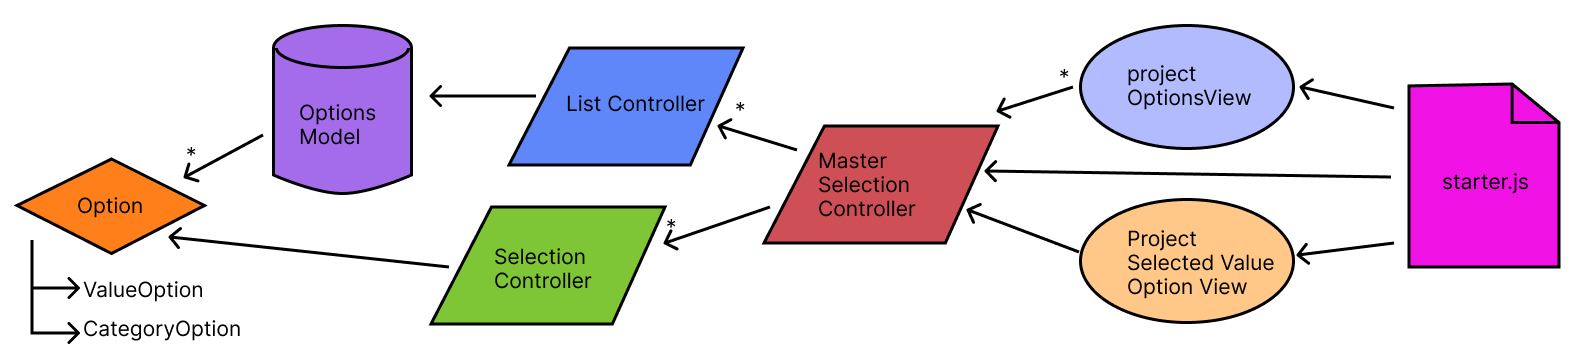
\includegraphics[width=120mm]{diagram-select-component-old.png}
    \caption{Diagramm Select Component - 1. Version}
    \label{Abbildung:DiagramSelectComponentOld}
\end{figure}

\begin{figure}[!htb]
    \centering
    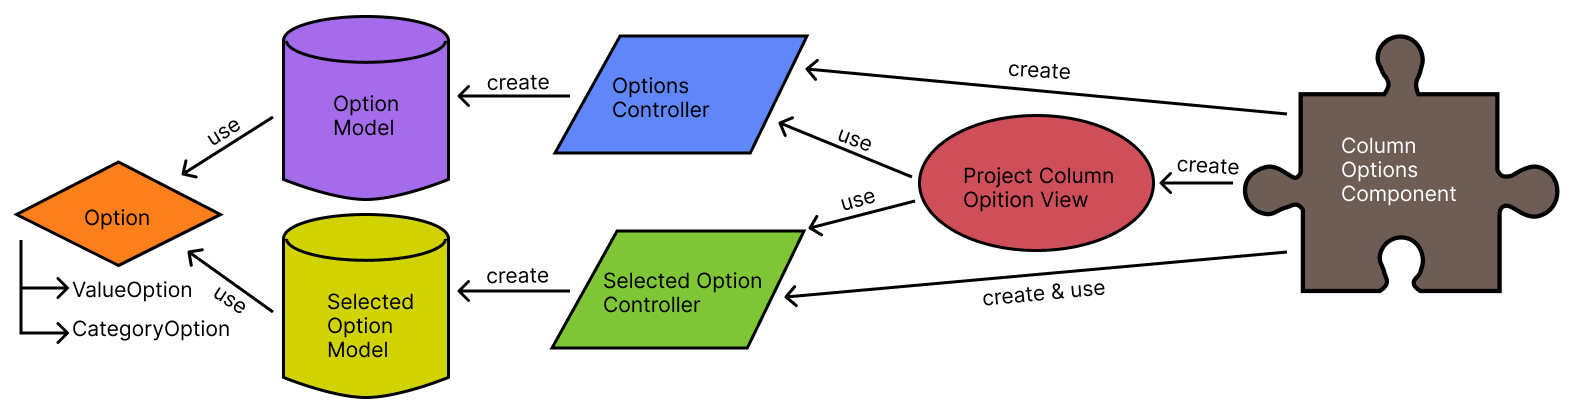
\includegraphics[width=120mm]{diagram-column-component-with-desc.png}
    \caption{Diagramm Column Component}
    \label{Abbildung:DiagramColumnComponent}
\end{figure}

\begin{figure}[!htb]
    \centering
    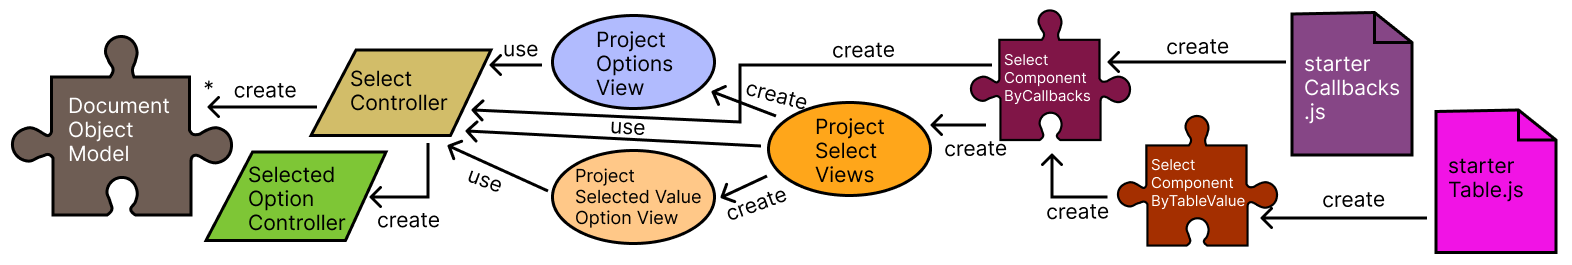
\includegraphics[width=120mm]{diagram-select-component-with-desc.png}
    \caption{Diagramm Select Component}
    \label{Abbildung:DiagramSelectComponent}
\end{figure}

\subsection{Popover}

% popover api 2024
% dialog popup


% entscheidungen
% kein filtern, keine suche => nicht unbedingt sortierte werte

\subsection{Performance}

Um eine gute Performance zu bieten, ist es notwendig den Aufbau-Prozess einer Webseite zu kennen.
Dieser Ablauf ist im Kapitel \textbf{Grundalgen} unter \textbf{Ablauf Parsing \& Rendering} genau beschrieben.
Die folgende Abbildung \ref{Abbildung:RenderingProcessRecap} zeigt den Prozess im Überblick.

\begin{figure}[!htb]
    \centering
    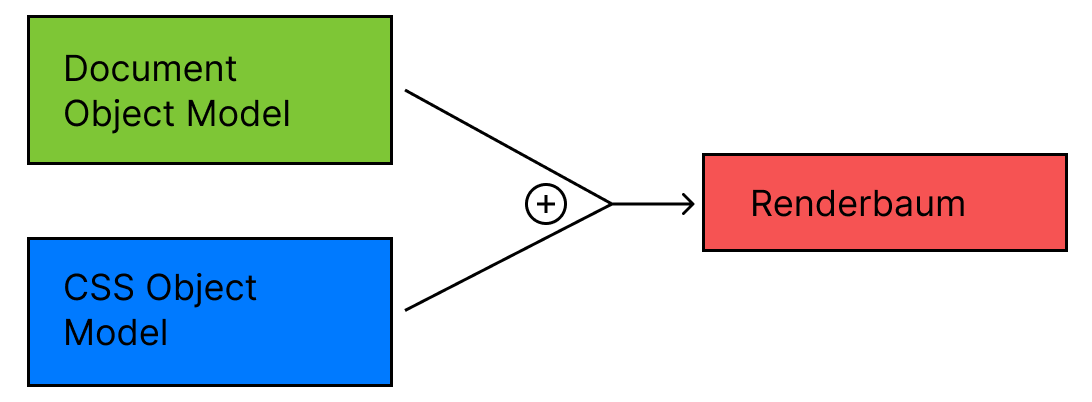
\includegraphics[width=120mm]{rendering-process.png}
    \caption{Rendering Prozess}
    \label{Abbildung:RenderingProcessRecap}
\end{figure}

Hierbei ist ein wichtiger Punkt, dass der Browser den Renderbaum (in der Abbildung \ref{Abbildung:RenderingProcessRecap} rot) maximal 60 Mal pro Sekunde neu zeichnen kann.
Daher müssen viele kleine Änderungen ausserhalb des Renderbaums - am besten in einem sogenannten Shadow-DOM - geschehen.
Ein Shadow-DOM ist ein Teilbaum, welcher nicht im Renderbaum angehängt ist.
Um dies zu bewerkstelligen, ist es sinnvoll, die Änderungen nach dem Abhängen des Elternknotens zu vollziehen. 
Nach den Änderungen kann der Teilbaum wieder an den gewünschten Ort platziert werden.

\begin{lstlisting}[language = java, caption = Code: Performance Optimierung (columnOptionsComponent.js), label = code:PerformanceOptimization]
    const addAllOptions = (options) => {
        const placeHolder = createHolder();
        columnView.replaceWith(placeHolder);
        if (options.length > 50) {
            setTimeout(() => {
                options.forEach((option) => {
                    optionsController.addOption(option);
                });
                updateScrollbar(columnView);
                placeHolder.replaceWith(columnView);
            }, 80);
        } else {
            options.forEach((option) => {
                optionsController.addOption(option);
            });
            updateScrollbar(columnView);
            placeHolder.replaceWith(columnView);
        }
    };
\end{lstlisting}
Code \ref{code:PerformanceOptimization} ist eine Stelle, die diese Technick verwendet.
Hier wird ein Platzhalter mit einem Lade-Indikator an die Ursprungstelle gesetzt, damit der Nutzer ein Feedback erhält.
Sobald der SpaltenContainer abgekoppelt ist, lädt die Funktion die Optionen in den Shadow-DOM.
Nach Abschluss wird der Container mit den neuen Elementen an die originale Stelle zurückersetzt.

(\cite{efficientDomManipulation}) Weiter kann auf 

\subsection{User Tests}


\subsubsection{Programmierer}



\subsubsection{Formular-Ausfüller}



% Keyboard navigation. Using keyboard to narrow down possible categories/values (maybe fuzzy searching), otherwise it takes me longer to find something than compared to a standard dropdown, even if the list there is bigger.
% Teams Nachricht an Lea ;)
% ich finde es etwas unintuitiv beim SelectComponent neben den offensichtlich verständlichen selectAttriutes (labl, name, numberOfColumns) noch ein Callback mitzugeben.

% ich hätti mir mehr beschreibung gewünscht wie ich die komponente verwenden muss. (ich musste eher dannach suchen.
% Bessere Dokumentation war verwirrend (Code).
% - Doku: In der Code Doku von SelectComponent dürfte der Return Value besser beschrieben werden (welches Array Element ist was). Das wird erst in den Anwendungsbeispielen klar.
% - Detail: numberOfColumns ist etwas "verbose"
% Es würde helfen, wenn die Types im JSDOC spezifiziert wären und wenn die Library eingebunden wäre. Dann wäre die Dokumentation leichter auffindbar.
% War mir am Anfang nicht klar dass was SelectComponent() zurückgibt und ob das Input-element sowie dass label-element selbst erstellt werden soll. Danach war es intuitiv anzuwenden.

% ---------

% Nitpicking: while I see why the component is imported from a URL for the user tests, it makes it hard to use on a spotty network.
% ich persönlich hatte zu beginn schwierigkeiten zu verstehen wie das "framework" funktioniert. die beschreibung für die tasks (ab task2) sind zum teil etwas unklar =>

% The value data is provided by the function `Service.getRegionsByCountry()`,
% the categories are provided by the function `Service.getCountries()`

% RegionsByCountry muss man noch das Country mitgeben. Hätte in der beschreibung drinstehen können.

\subsection{Diskussion}

% herausforderungen
% komplexeste probleme
% erfolge
% unerwartete wendungen

\subsection{Fazit}
